\section{Results}
\label{exp}
Our experiments are organized in the following way.
We first evaluate our approach on a synthetic benchmark dataset where we can control the data distribution and the update rate.
Our first experiment will discuss the practical overheads and tradeoffs to using our approach.
Then, for three specific materialized views, we evaluate accuracy, performance, and outlier indexing.
After evaluation on the benchmark, we present an end-to-end application of log analysis with a dataset from Conviva.
Conviva is a video streaming company that logs activity for each of their videos such as who is watching the video, who owns the video, browser, and network latency etc. 

We define the following metrics for evaluation.
For accuracy, we measure the relative error between estimated query result and the true query result.
A relative error of 5\% means that the difference between the estimated query result and the true result is 5\% of the true result.
As baselines, we compare against two alternative approaches, no maintenance where the materialized view is left to be stale and SAQP where instead 
of calculating an approximate query correction we estimate directly from the up-to-date view.
We fix the sampling ratio of SAQP and our approach to be the same so they will have the same maintenance time.
Even so, SAQP as defined, requires more storage than our approach.
For performance, we measure the maintenance time as the time required to calculate the delta view and then refresh the materialized view for a batch of updates.
We also measure query execution time as the time taken from issuance of a query to completion.
As a baseline, we compare the performance to full incremental maintenance.
The measured time is the ``wall clock" time and this is measured with no other load on the server.

\subsection{Experimental Setting}
\subsubsection{TPCD-Skew}
The first dataset, TPCD-Skew dataset, is based on the Transaction Processing Council's benchmark
schema but is modified so that it generates a dataset with values drawn from a Zipfian powerlaw distribution instead of uniformly.
The Zipfian distribution [?] is a long-tailed distribution with a single parameter $z=\{0,1,2,3,4\}$ which a larger
value means a more extreme tail.
This database has been applied to benchmark other sampling based approaches and outlier performance [?].
The dataset is provided in the form of a generation program which can generate both the base tables and a set of updates.

For this dataset, we applied our approach to three materialized views, each of a different type:
\vspace{1em}

\textbf{Select-Project View}
\begin{lstlisting}
SELECT *, 
     if(lcase(l_shipinstruct) 
     	     LIKE '%deliver%' 
        AND lcase(l_shipmode) 
             LIKE '%air%',
                  'priority',
                  'slow') 
FROM lineitem_s
\end{lstlisting}

\vspace{1em}

\textbf{Aggregation View}
\begin{lstlisting}
SELECT l_orderkey, 
       l_shipdate, 
       sum(l_quantity) as quantity_sum, 
       sum(l_extendedprice) as extendedprice_sum, 
       max(l_receiptdate) as receiptdate_max, 
       count(*) as group_count 
FROM LINEITEM 
GROUP BY l_orderkey, l_shipdate
\end{lstlisting}

\vspace{1em}

\textbf{Foreign-Key Join View}
\begin{lstlisting}
SELECT supplier.*, 
	   customer.* 
FROM   customer, 
       orders, 
       lineitem, 
       supplier, 
       partsupp 
WHERE  c_custkey = o_custkey 
   AND o_orderkey = l_orderkey 
   AND l_suppkey = ps_suppkey 
   AND l_partkey = ps_partkey 
   AND ps_suppkey = s_suppkey 
   AND s_nationkey <> c_nationkey
\end{lstlisting}

\vspace{1em}

The base dataset we generated is 10GB corresponding to 60,000,000 records, and the above three views are derived from this base dataset.
For these three views, we randomly generated aggregation queries and evaluated them for different sample sizes, different update rates, and different parameter settings for the Zipfian distribution.
All of our experiments for the TPCD-Skew dataset are run on a single r3.large Amazon EC2 node with a MySQL database.

\subsubsection{Conviva}
Conviva is a video streaming company and we evaluated our approach on user activity logs. 
We experimented with a 1TB dataset of these logs and a workload corresponding analyst queries on the log.
We used this dataset to evaluate the end-to-end accuracy and performance of the system on a real dataset and query workload.
We evaluated performance on Apache Spark with a 20 node r3.large Amazon EC2 cluster. 


\subsection{Update Rate and Accuracy}
In the first experiment, for each of the three views listed above, we evaluate the accuracy of our approach.
We measure accuracy by using the average relative query error for a set of 10000 randomly generated queries on each view.
We set the sample size to $5\%$ and then vary the number of inserted records by increments of 500000 records to a final count of 8000000 records (1.3GB).
We evalute SAQP and our approach against a baseline stale result.
In Figure \ref{exp2udpate}, we show the results of the experiment. 

\begin{figure*}[ht!]
\label{exp2update}
\centering
 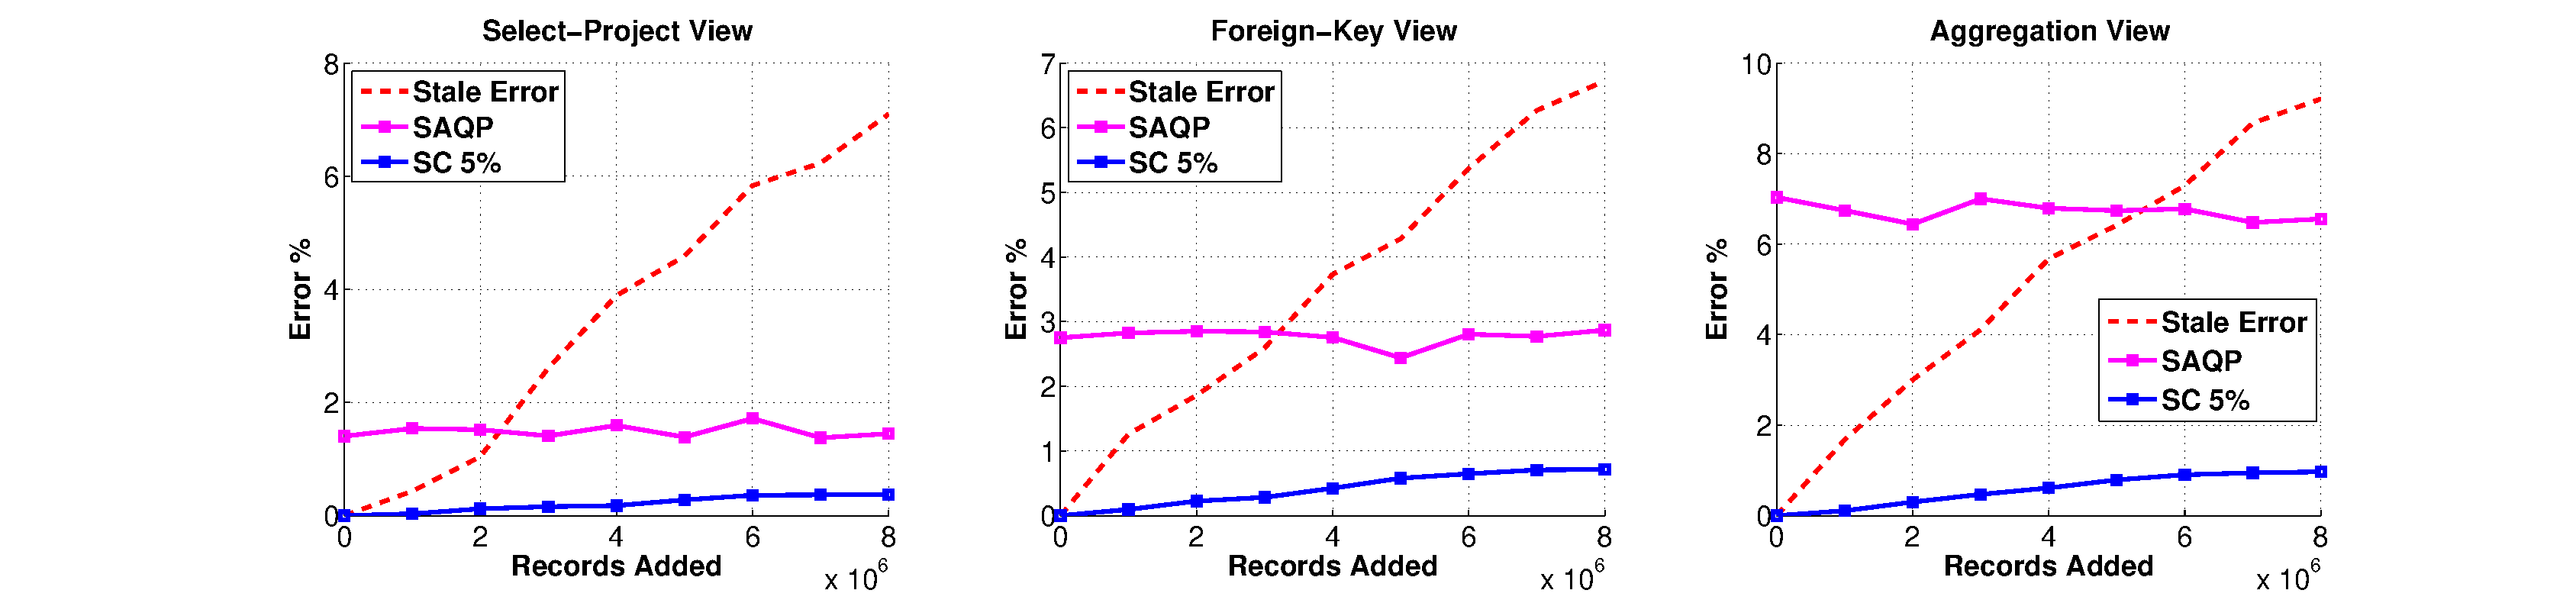
\includegraphics[width=\textwidth]{exp/exp2-updatesize-accuracy.eps}
 \caption{TODO}
\end{figure*}

The results highlight an important point comparing the accuracy of SAQP to our approach. 
The accuracy our approach is proportional to the amount of correction needed, while SAQP keeps a roughly constant accuracy.
As more records are inserted the approximation error in our approache increases.
However, we find that even for very large amounts of inserted records (>10\% of dataset size), our approach gives significantly more accurate results
than SAQP.
The gain is most pronounced in aggregation views where there are a mixture of updated and inserted rows into the view.
Compensating for a correction to an existing row is often much smaller than doing so for a new inserted record.


\subsection{Computational Efficiency}
In the next experiment, we evaluate how sampling can reduce maintenance time.
For a batch of updates, we evaluate how long it takes to incrementally maintain a view compared to maintaing a sample.
For, the join view, we build an index on the foreign key of the view.
As before, we derived the views from a 10GB base dataset, and inserted records in increments of 500000.

\begin{figure*}[ht!]
\label{exp3dist}
\centering
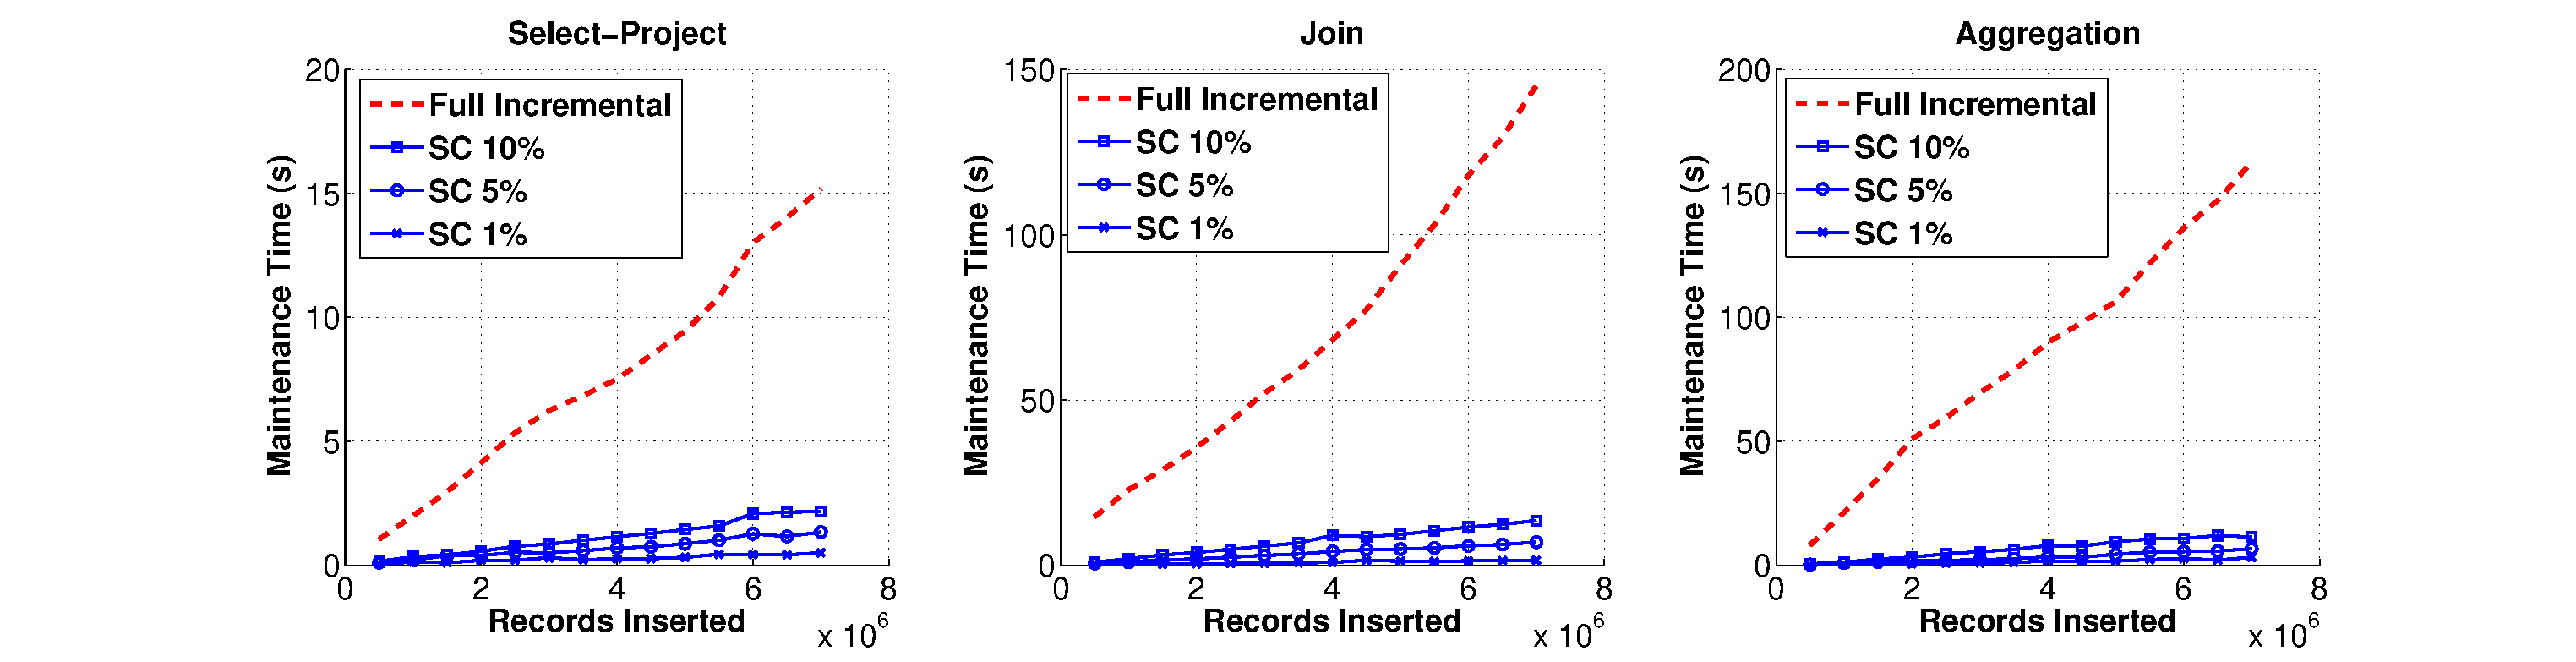
\includegraphics[width=\textwidth]{exp/exp4-efficiency-tpcd-skew.eps}
 \caption{(placeholder) TODO}
\end{figure*}

We find that maintaining a sample is far cheaper than the entire view. In this experiment, keeping a view exactly up-to date required computation on the order of minutes.
However, we found that with a small sample we could acheive this in a few seconds and still acheive accurate results.

\subsection{Overhead of Query Correction}
In Section \ref{sampling}, we ran cost analyses to argue that sampling can greatly reduce delta view and refresh costs.
Furthermore, in the previous experiment, we showed that for the three specific views sampling can greatly reduce maintenance time.
In practice, these gains will only be meaningful if the overheads for the query correction are small.
Since, we are correcting a stale query rather than the materialized view, we are shifting some of the computational cost from maintenance time to query execution time.
For Select-Project and Foreign-Key join views, since we derive a correction from a sample of the updates, we are guaranteed to have 
a reduced query time. \reminder{SK: This may not be true due to deletions}
However, for aggregation views, query correction requires a scan of the old view and a sample of the maintained view; potentially increasing the time to 
answer the query.
In our first experiment, we set the sample size to 5\% and evalute the aggregation view listed earlier for 5000000 inserted records. 
In (Figure \ref{exp10overheads}), we show that average query time is small compared to maintenance time, and furthermore, 
the time to calcuate a correction is a just fraction of the query time.
\begin{figure}[h]
\label{exp10overheads}
\centering
 \includegraphics[width=\textwidth]{exp/total_time_agg_view.pdf}
 \caption{TODO}
\end{figure}

\subsection{View Complexity}
Another question is how expensive view maintenance needs to be before our approach becomes worthwile.
We evaluated this by taking the simplest possible view, a SELECT of the base table, and then progressively adding clauses to the predicate.
For example:
\begin{lstlisting}
WHERE (condition1)
WHERE (condition1 || condition2)
WHERE (condition1 || condition2 || condition 3)
\end{lstlisting}
We set the sample size to 5\% and measure the maintenance time.
For a such a view, the only cost for maintenance is a scan of the data and evaluating the predicate. 
Sampling saves on predicate evaluation but introduces the overhead of random number generation.
Figure \ref{exp11overheads} illustrates how as the view becomes for complex the performance improvement given
by our approache increases.
Initially, the random number generation adds about 5\% overhead, but as the cost of evaluating the benefits increase.
We repeated the same experiment for the aggregation view, but instead we added terms to the group by clause to increase the
cardinality of the view.
We found that for a highly selective group by clause (thus a large view) the savings were nearly perfect (20x).
However, when the view was small the cost savings were smaller.
\begin{figure}[h]
\label{exp11overheads}
\centering
 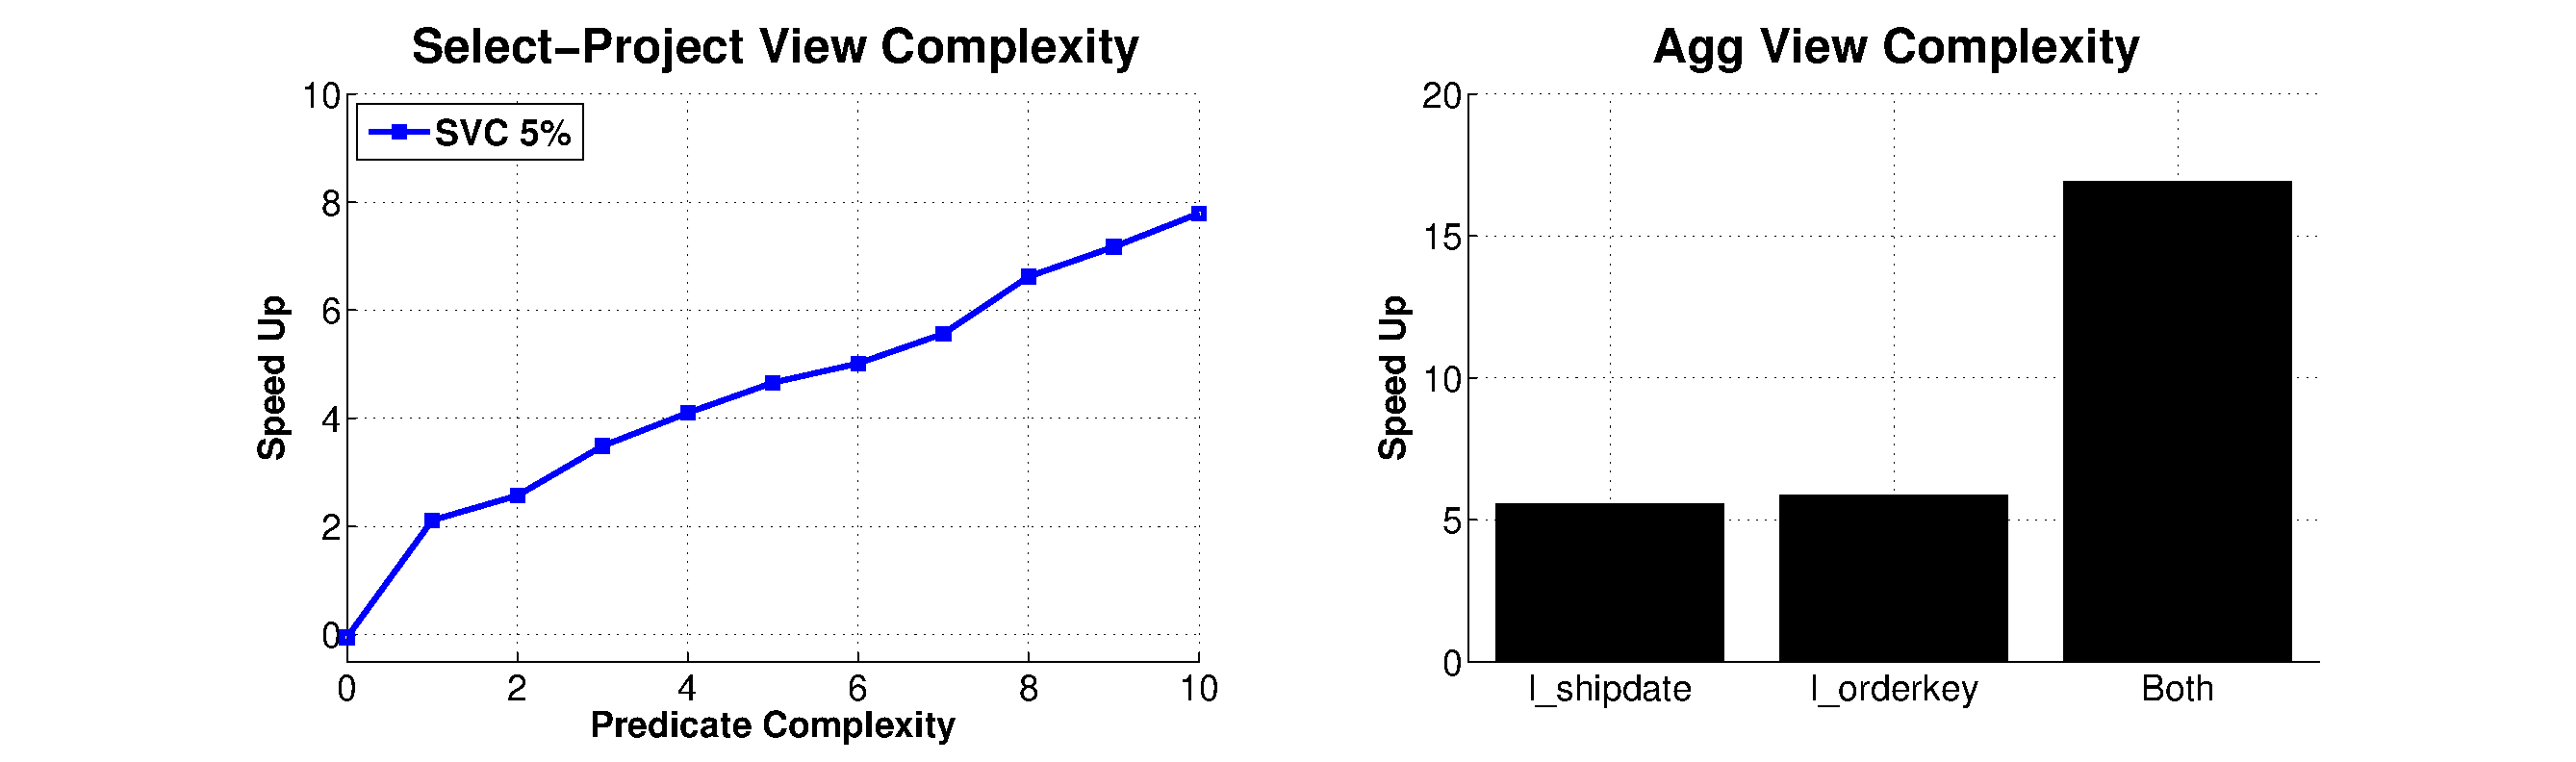
\includegraphics[width=\textwidth]{exp/complexity_efficiency_tradeoff.eps}
 \caption{TODO}
\end{figure}
This experiment emphasizes that our approach rareley makes performance worse and at worst the improvements are not linear with the sampling ratio.
Furthermore, we emphasize that when views are large and complex, as often the case, we can have significant improvements.

\subsection{Outlier Indexing}
We ran experiments on the TPCD-skew dataset to evaluate how outlier indexing can improve the accuracy of our approach without adding much overhead.
In the first experiment, we evaluate the accuracy for each of the views as a function of the size of the outlier index. 
We use a 5\% sample size and 5000000 records inserted, and we evaluate the accuracy of our approach with and without outlier indexing.
In the Select-Project view, we index the attributes l\_extendedprice and l\_quantity.
For the Join view, we index the attributes customer.c\_acctbal and supplier.s\_acctbal.
Finally, in the Aggregation view, we index the attribute l\_extendedprice.

In the first experiment, we varied the total number of indexed records and plot accuracy as a function of index size.
As a baseline, we compare if the same number of records were randomly sampled.
In Figure \ref{exp7outlier}, we find that outlier indexing can improve accuracy by a factor of three for the join view. 
In the same figure, we break down for which queries these gains are made. 
We find that outlier indexing addresses the most inaccurate queries as these are often due to outliers. 
\begin{figure*}[ht!]
\label{exp7outlier}
\centering
\includegraphics[width=\textwidth]{exp/exp6-outlier.eps}
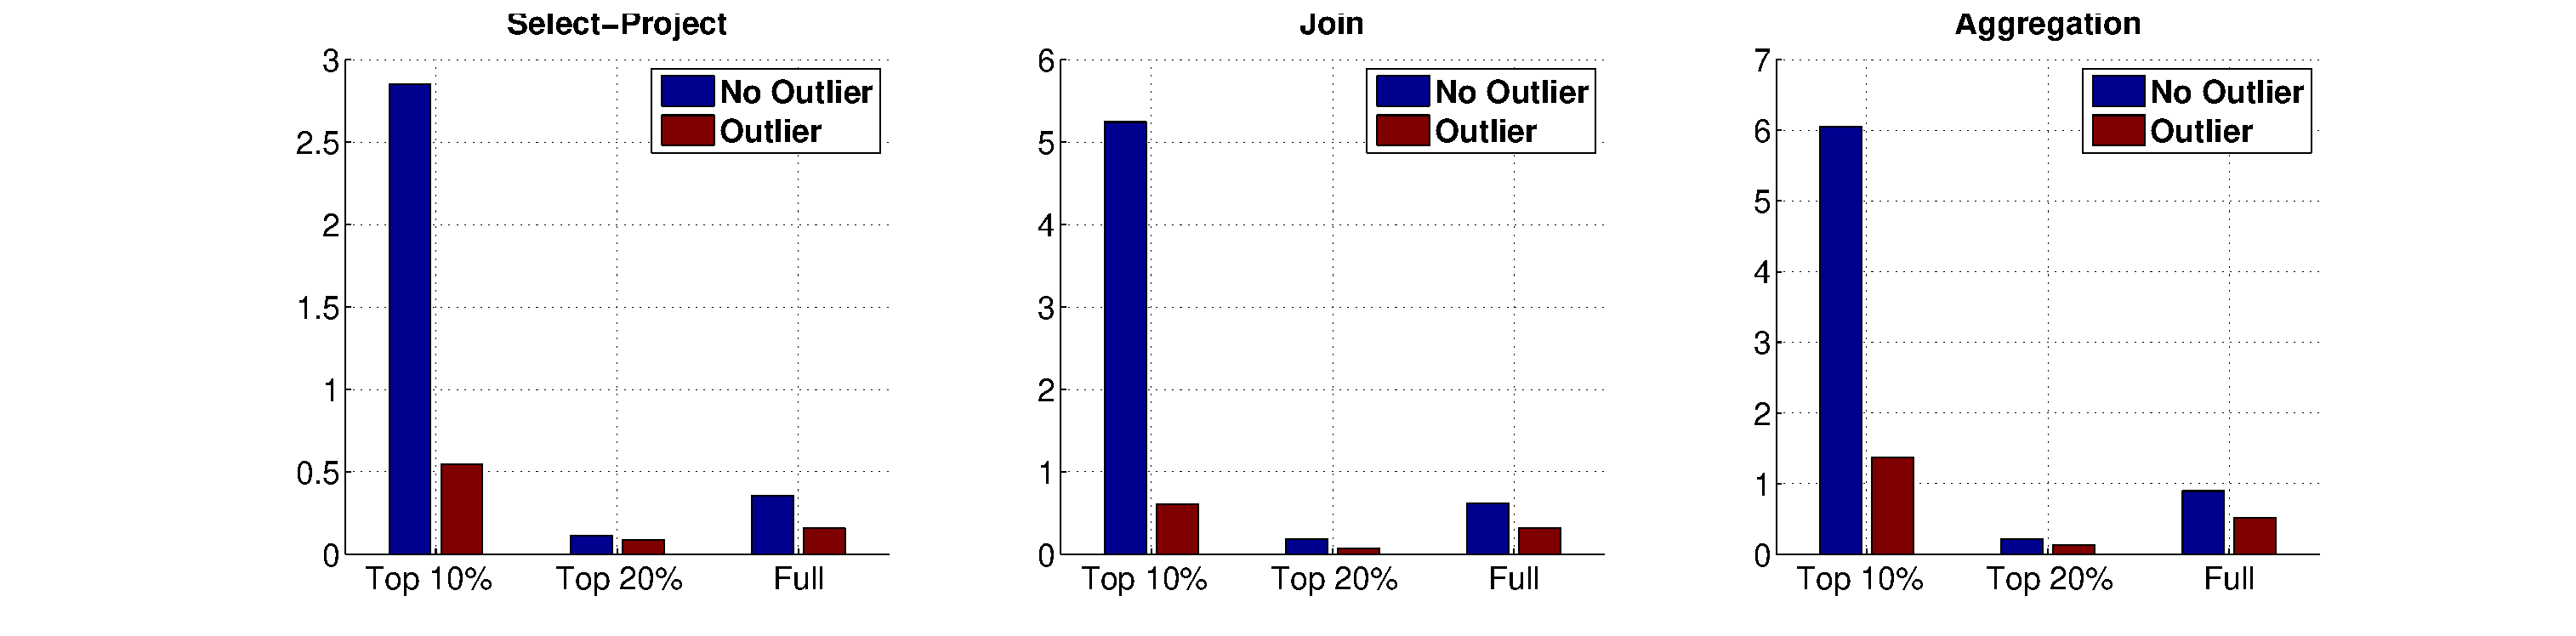
\includegraphics[width=\textwidth]{exp/exp7-outlier.eps}
 \caption{(placeholder) TODO}
\end{figure*}

Next, we evaluated how the approach works under different levels of skew in the dataset. We varied the Zipfian parameter from (0,1,2,3,4) and measured the average improvement in accuracy. 
We found that as the dataset become more skewed, outlier indexing is increasingly important.
\begin{figure*}[ht!]
\label{exp8outlier}
\centering
\includegraphics[width=\textwidth]{exp/exp8-outlier.eps}
 \caption{(placeholder) TODO}
\end{figure*}

Finally, we evaluated the overhead for the approach. 
We found that small indicies were sufficient for good accuracy and thus the additional overhead was marginal and orders of magnitude smaller than sample maintenance time.

\begin{figure*}[ht!]
\label{exp9outlier}
\centering
\includegraphics[width=\textwidth]{exp/exp9-outlier.eps}
 \caption{(placeholder) TODO}
\end{figure*}

\subsubsection{Distribution of Query Error}
In our earlier experiments, we presented the average error for the queries on the views.
In this experiments, we looked at the distribution of query errors and compared that to their staleness.
For each of the three views, we derive the views from a 10GB dataset.
Then, as before, we simulate 5000000 inserted records and a 5\% sample.
We evaluated the relative error for each query.

\begin{figure*}[ht!]
\label{exp3dist}
\centering
 \includegraphics[width=\textwidth]{exp/exp3-query-error-dist.eps}
 \caption{TODO}
\end{figure*}

In Figure \ref{exp3dist}, we present staleness vs. estimation accuracy as a scatter plot.
For all three of the views, the median error is greater than 10 times less than the staleness. 

However, this distribution motivates our outlier indexing as there are clearly outlier queries.
Outliers can occur for a variety of reasons.
First, some of the generated queries are highly selective and a uniform sampling approach may not sample enough records to answer it accurately.
Next, outliers can be caused by large updates to the data that are missed by our sampling.
In Section ?, we show how outlier indexing can solve the latter problem and, in fact, after outlier indexing all of our queries on these three views are estimates more accurately than the pre-existing staleness error.

\subsection{Sample Size and Accuracy}
In this experiment, we illustrate the tradeoff between sample size and accuracy.
For each of the three views, we evaluate average query accuracy as a function of sample size.
Then, we simulate 5000000 inserted records, corresponding to about 800MB.
We then vary the sampling ratio for the three types of views and show how much sampling is needed to acheive a given query accuracy.
For 10,000 randomly generated aggregation queries on each view, we compare the stale query error to SAQP and our approach.
For SAQP and our approach, we keep the same sampling ratio.
This does, however, mean that SAQP uses significantly more storage than our approach Select-Project and Foreign-Key Join Views.

\begin{figure*}[ht!]
\label{exp1sample}
\centering
 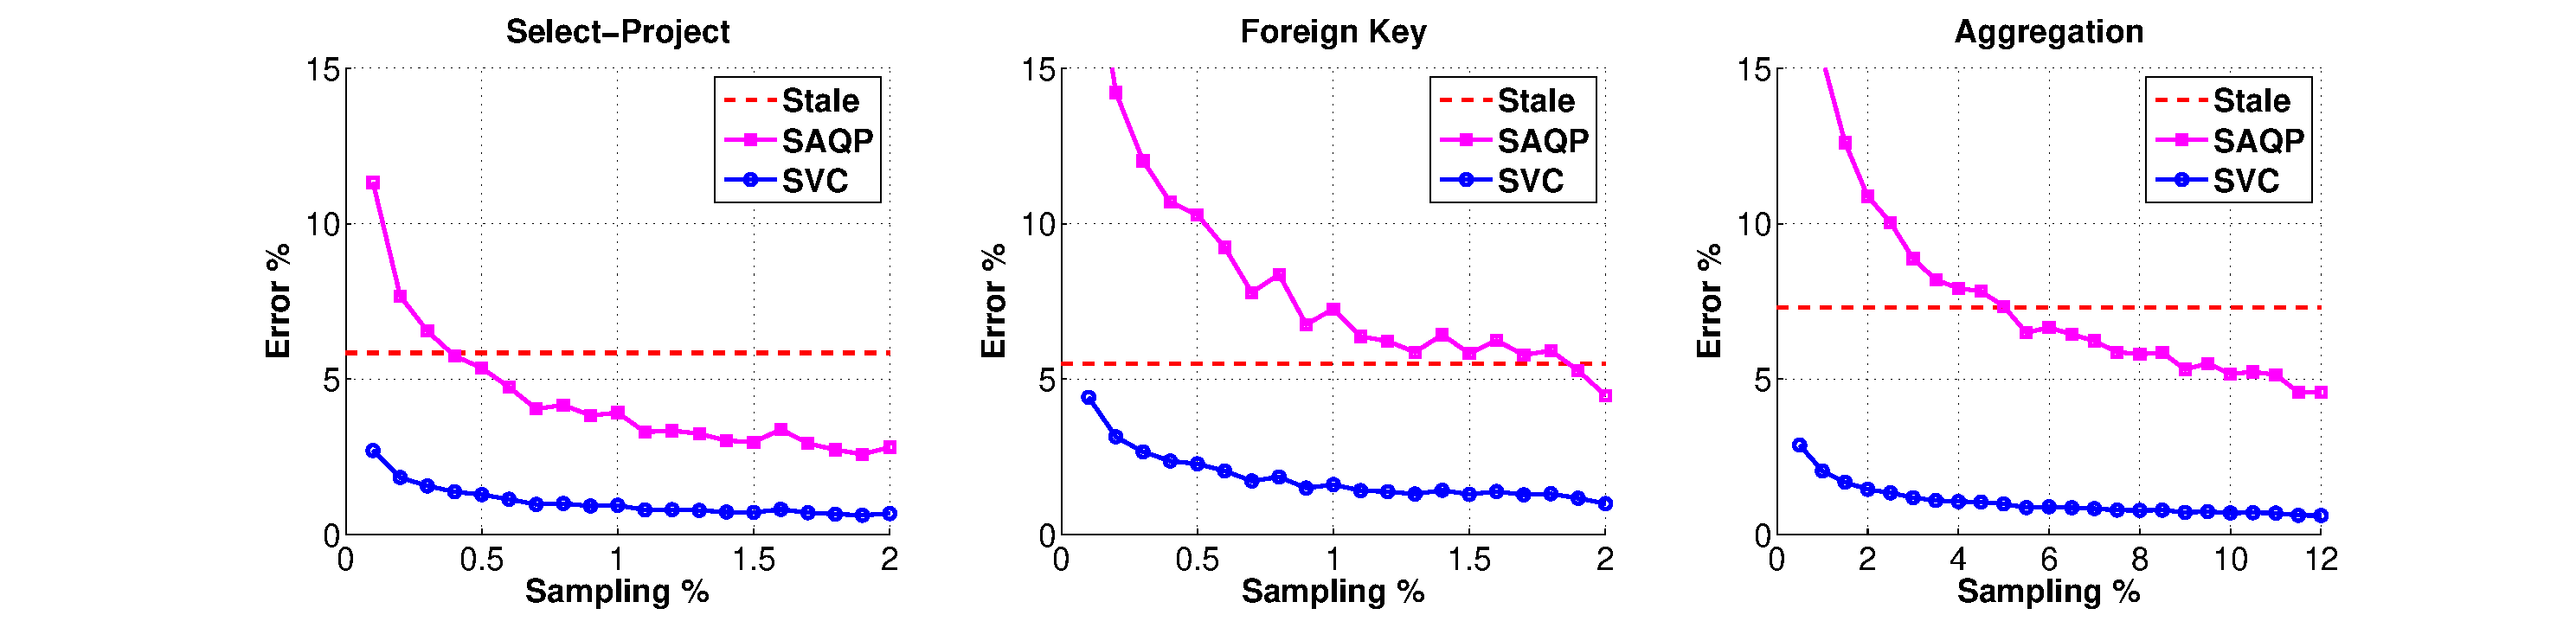
\includegraphics[width=\textwidth]{exp/exp1-samplesize-accuracy.eps}
 \caption{TODO}
\end{figure*}

In Figure \ref{exp1sample}, we show the accuracy as a function of sampling ratio for each of the views.
For both SAQP and our approach, there is a break-even point at which the approximation error is less than the staleness error.
At sampling ratios beyond this point, our query approximated queries are on average more accurate than queries on the stale view.
For all three of the views, the average query error is significantly less than SAQP as the break-even point happens earlier in our approach.

\subsection{Application: Log Analysis For Conviva}
We used a dataset of queries given by Conviva to generate three materialized views:
\vspace{1em}

\textbf{View 1}
\begin{lstlisting}
SELECT clientId, 
       customerId, 
       sessionTimeMs, 
       count(1) 
         as group_count, 
       max(sessionTimeMs) 
         as sessionTimeMs_max, 
       avg(lastBufferLengthMs) 
         as lastBufferLengthMs_avg,
       avg(lLifePausedTimeMs) 
         as lLifePausedTimeMs_avg 
FROM anon_sdm2_ss 
GROUP BY clientId, customerId
\end{lstlisting}

\vspace{1em}

\textbf{View 2}
\begin{lstlisting}
SELECT customerId, 
       sessionType, 
       count(1) as group_count, 
       max(estBwCount) 
           as estBwCount_max, 
       sum(buffTimeMs) 
           as buffTimeMs_sum, 
       sum(estBwCount) 
           as estBwCount_sum 
FROM anon_sdm2_ss 
GROUP BY 
customerId, sessionType
\end{lstlisting}

\vspace{1em}

\textbf{View 3}
\begin{lstlisting}
SELECT justStarted, 
       sessionType, 
       startResourceState, 
       state, 
       count(1) 
            as group_count, 
       max(playTimeMs) 
            as playTimeMs_max, 
       min(stoppedTimeAtJoinMs) 
            as stoppedTimeAtJoinMs_min, 
       max(lifeAverageBitrateKbps) 
            as lifeAverageBitrateKbps_max 
FROM anon_sdm2_ss 
GROUP BY justStarted, 
         sessionType, 
         startResourceState, 
         state
\end{lstlisting}

All three of these views are aggregation views. 
View 1 has the most selective group by clause and was chosen to a be a large view where most of the maintenance is in the form of new rows to insert.
View 2 is a medium size view where maintenance is a mix of both updates and insertions.
View 3 is a small view where most of the maintenance is updates to existing rows.
For these views, we randomly generated aggregation queries.

\subsubsection{View Selection}
We selected these views to be representative of the dataset and query workload. 
We first present an experiment illustrating where these materialized views lie in the space of all the generated views.
We derived each view from a 7GB base table and inserted 1.5GB of records to the table. 
On a single node, we evaluated the average query accuracy for a 1\% sample and the runtime of our approach.
In Figure \ref{exp12conviva}, we plot the three views on the distribution of error and runtime and we see that they 
are from different parts of the distribution.
\begin{figure}[ht!]
\label{exp12conviva}
\centering
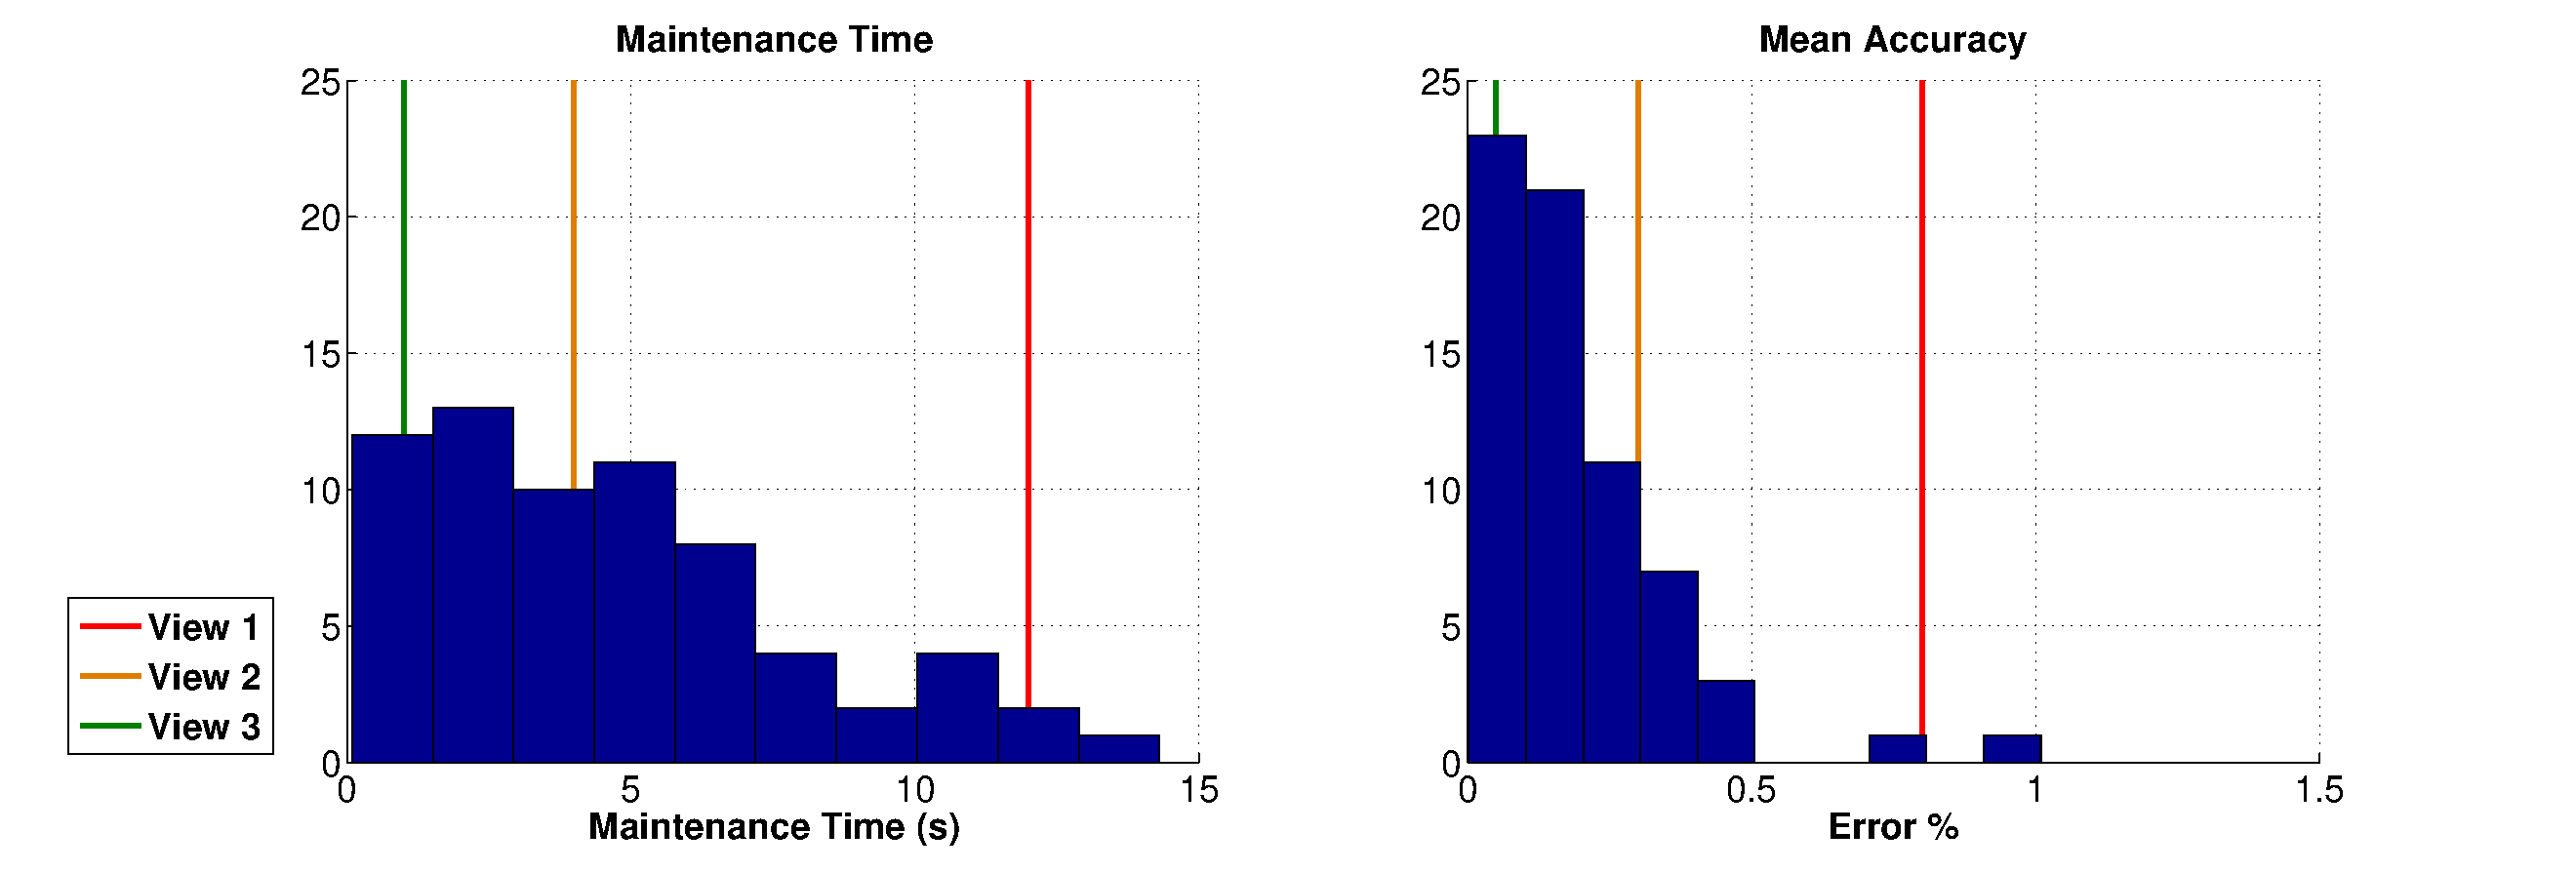
\includegraphics[width=\textwidth]{exp/conviva_efficiency_accuracy.eps}
 \caption{TODO}
\end{figure}

\subsubsection{Accuracy in Conviva}
We evaluated the average query accuracy for different sample sizes and numbers of records inserted.
As before, we derived each view from a 7GB base table and inserted 1.5GB of records to the table. 
We built an outlier index on all of the attributes that represent time intervals or rates (buffTimeMs, stoppedTimeAtJoinMs, playTimeMs, lifeAverageBitrateKbps).
Figure \ref{exp5conviva}, compares the accuracy to the staleness of the query.
We find that even a $0.1\%$ sample gives significantly more accurate results for View 1 and View 2.
Even in the situation where the view is small, sampling can still have benefits as seen in View 3.

\begin{figure*}[ht!]
\label{exp5conviva}
\centering
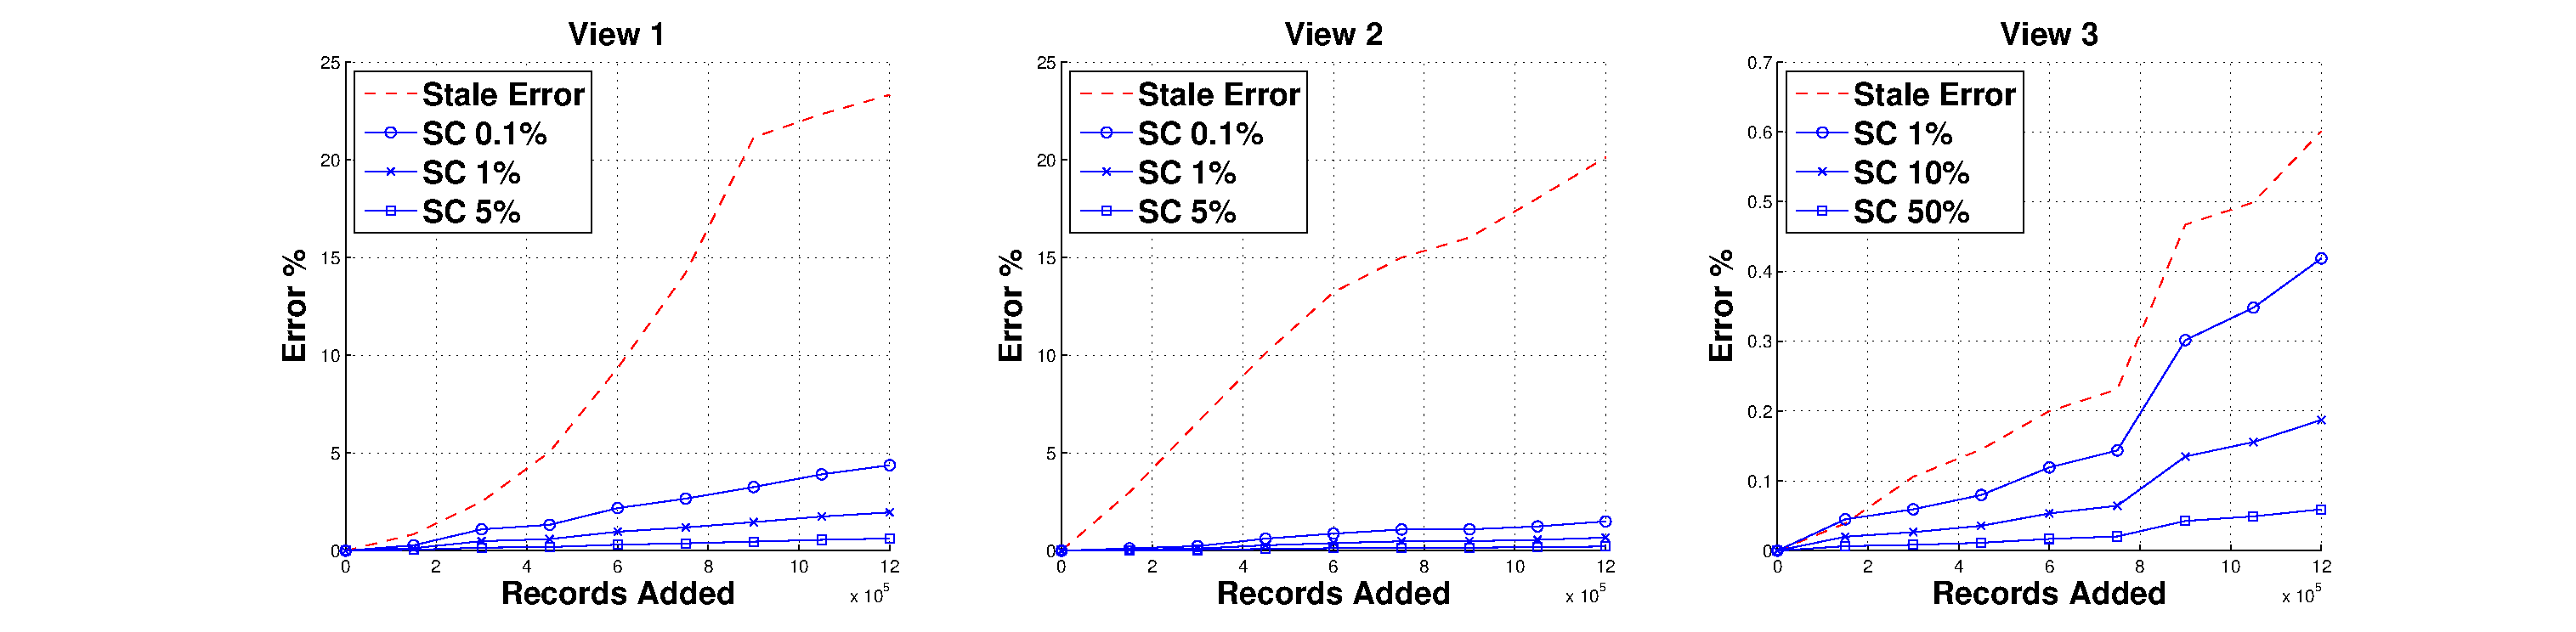
\includegraphics[width=\textwidth]{exp/exp5-coniva-accuracy-woutlier.eps}
 \caption{TODO}
\end{figure*}

\subsubsection{Performance in Conviva}
We evaluated performance on Apache Spark, on a 20 node r3.large Amazon EC2 cluster. 
This cluster had enough memory to hold all of the materialized views in memory.
Spark supports materialized views through a distributed data structure called an RDD [?].
The RDD's are immutable, thus requiring significant overhead to maintain.
We compare maintenance to recalculation of the view when the data is in memory and when only the updates are in memory. 
We derived the views from a 120GB base relation and inserted records in 10GB increments.
As Spark does not have support for indices, we rely on partitioned joins for incremental maintenance of the aggregation views.
Each view is partitioned by the group by key, and thus only the sampled delta view has to be shuffled. 

\begin{figure*}[ht!]
\label{exp6conviva}
\centering
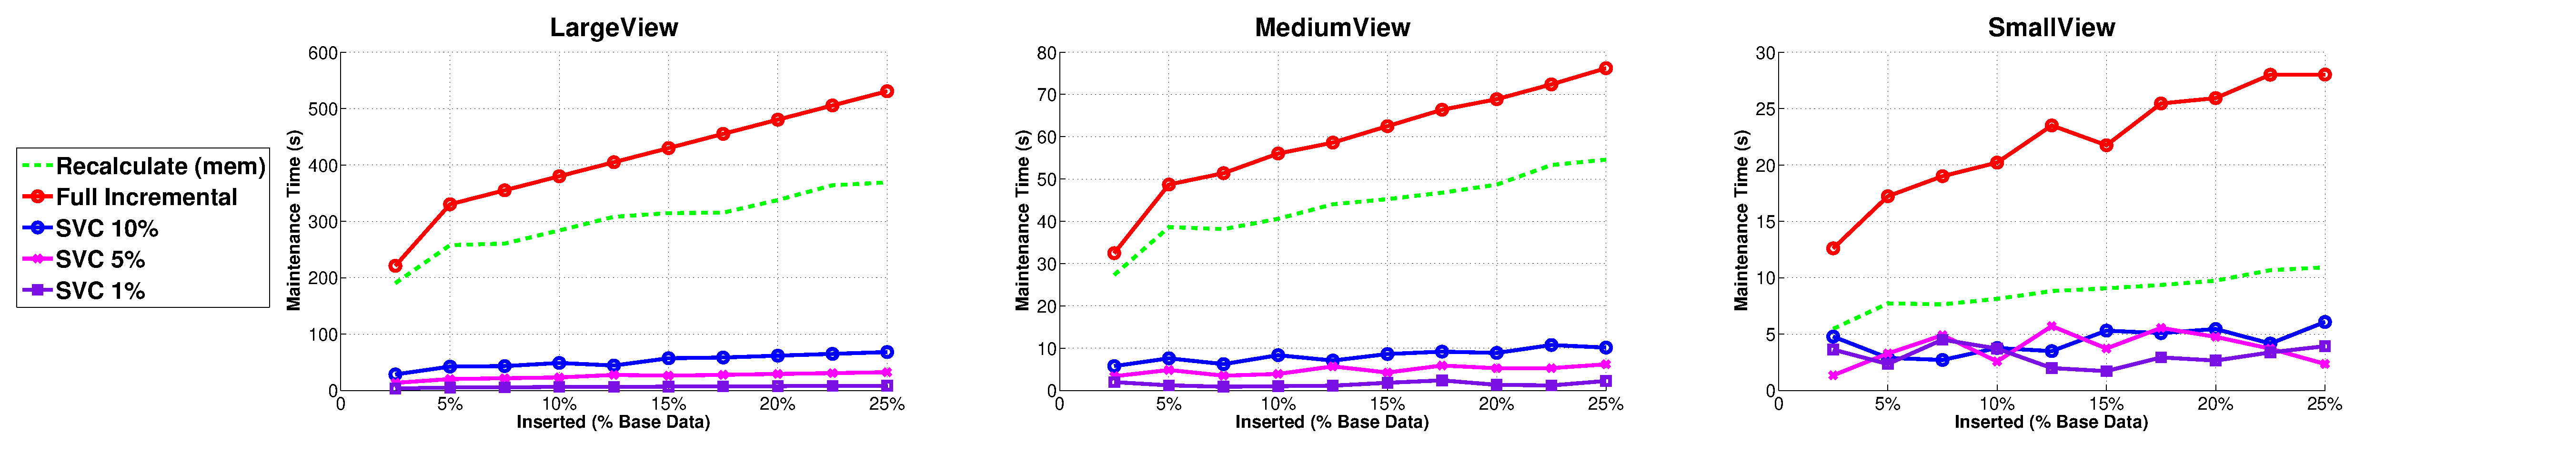
\includegraphics[width=\textwidth]{exp/exp5-efficiency-conviva.eps}
 \caption{(placeholder) TODO}
\end{figure*}

In Figure \ref{exp6conviva}, we illustrate the maintenance time as a function of the number of inserted records.
We find that we acheive good scalability on view 1 and view 2, and still have some performance gains on view 3.
In view 1 and view 2, our gains are more pronounced due to the savings on communication in a distributed environment.
As view 3 is smaller, the communcation gains are less and the only savings are in computation.



